\chapterauthor{Camden Landis}

%\epigraph{Didn’t I tell you? I’ve got a brain the size of the planet. No one ever listens to me of course.}{Marvin the Paranoid Android, \emph{The Hitch-Hiker's Guide to the Galaxy}.}

\minitoc

\noindent This project's complete source code can be found at the following link:\\
\url{https://code.vt.edu/craine/aes-image-encryption} 
\vspace{-0.2in}

\section{Introduction}
The amount of confidential data that is transferred within functioning societies is enormous, so ensuring privacy and security of the data is paramount. Advanced Encryption Standard (AES) is one of the most popular and extensively used symmetric, private-key block ciphers in cryptography. In fact, it is the encryption standard used by the United States federal government for securing classified information. AES consists of different rounds of permutations and substitutions, all depending upon the key size used which can be 128-bit, 192-bit, or 256-bit in length.

One issue that the AES faces is that, while it is efficient to encrypt data when using a 128-bit key, it can be much more computationally slow when using larger key lengths such as 256-bit. Efficiently encrypting a high-resolution image requires a high relative processing time, so utilizing the parallelization of modern GPUs could increase time and throughput efficiency when encrypting an image (or batch of images). Specifically, images can be represented as a two-dimensional arrays of bit data allowing for straightforward thread-block design when structuring code in CUDA. This parallel implementation allows each core of the GPU to operate independently and simultaneously on segments of an image increasing the time and throughput efficiency of the AES.

\section{Literature Review}

Iwai, et al. present an in-depth look at implementing the AES with CUDA; their paper overviews granularity of AES parallel processing by analyzing the efficiency levels of varying thread-block designs \cite{Iwai2012}. They also examine the computational impact of S-Box and round key data storage on shared memory. Ma et al. discuss how the performance of an AES implementation based on GPUs is influenced by the size of input data, the number of threads per block, memory allocation style, and (similar to Iwai, et al.'s reseach) parallel granularity \cite{Ma2017}. Finally, Saxena, et al. present a parallel implementation of the AES using CUDA and OpenCV to encrypt images rapidly; their implementation achieved an average speed up of four times on GPU as compared to their CPU-only implementation \cite{Saxena2020}.

\section{AES Overview}
The AES is a symmetric block cipher introduced in 2002 by NIST based on the Rijndael standard developed by developed by two Belgian cryptographers Vincent Rijmen and Joan Daemen. The data length in AES is 128 bits (16 bytes). However, the key can acquire different lengths (for example, 128, 192, 256 bits). AES has 10, 12 and 14 rounds for 128-bit, 192-bit and 256-bit keys, respectively. Figure 1 shows the block diagram of the general AES algorithm.

\begin{figure}[h]
\centering
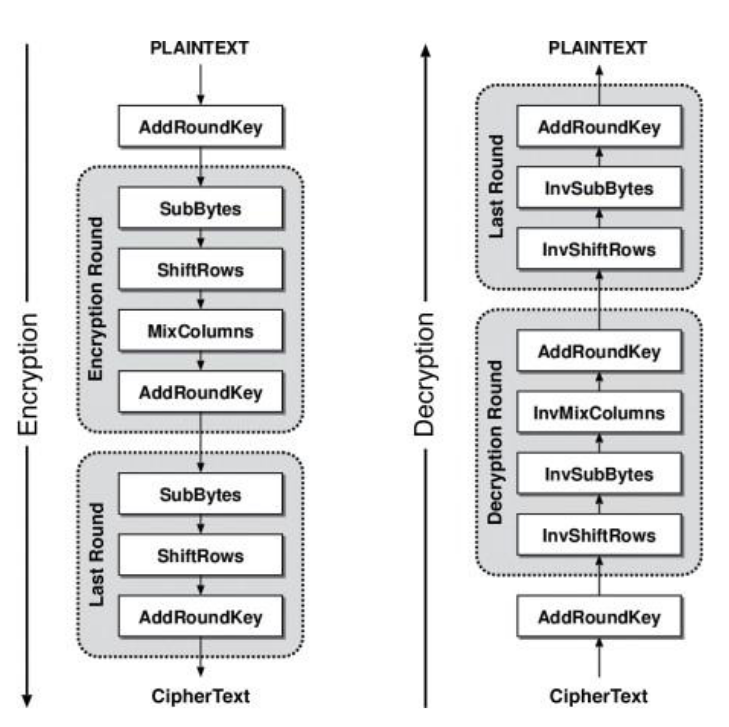
\includegraphics[scale=.4]{tex/Projects/CamdenLandis/aes-block-diagram.png}
\caption{General AES block diagram.}
\end{figure}

The AES has four main operational blocks:
\begin{enumerate}
    \item Byte substitution transformation (SubBytes): An S-box is used to substitute each data block byte with another block.

    \item Shift transformation of rows (ShiftRows): Each row of the state matrix is given a cyclic shift to the right side according to its location.

    \item Mix Transformation of Columns (MixColumns): It is a matrix multiplication operation where each column of the state matrix is multiplied by that of the fixed matrix.

    \item Add round key transformation (AddRoundKey): XOR operation is performed between the new state matrix and the round key one.
\end{enumerate}

\noindent In order to decrypt, one needs to perform all the operations in the reverse order and use the key schedule in reverse order. The operations ShiftRows, SubBytes, MixColumns, and AddRoundKey must be replaced by their inverse operations. 

\noindent It should be noted that as of right now, the AES is secure against all known attacks; in other words, there are no known attacks on AES that are faster than brute force exhaustive search which could potentially take billions of years on current hardware. GPU-enhanced parallel code could certainly decrease exhaustive search time, but the AES remains computationally secure with this considered.

\section{AES Parallel Implementation}
The actual components of each round in the AES block cipher are rather linear in nature, and parallelizing the round operations themselves may not improve throughput. This is due to the fact that the round operations must happen sequentially in order to replicate the AES algorithm, however, some parallelized round functions can be found online. On the other hand, the encryption and decryption operations can be parallelized. For my implementation, I considered the AES block size when deciding on my code's thread number and thread-block size.

\noindent Since the AES is a block cipher which operates on 128-bit of input at a single iteration, I divide the input image into 16 pixel block sizes. This means that 16 pixels of the image will be operated on by a single thread, and using 512 threads per block, 8,192 pixels will be processed by each thread-block. I also call \texttt{\_\_syncthreads()} after each operation to ensure the threads in each of the blocks are synced properly. For this project, I utilized the standard \texttt{bitmap.c} functions for inputting and storing bitmap image data. The \texttt{tools/} directories in the source repository for this project contain more information about usage.

\noindent The following (Listings 1 and 2) are my current encryption and decryption CUDA kernels both of which are utilizing shared memory:
\newpage
\begin{shaded} 
\begin{lstlisting}[language=C, caption={AES Encryption Kernel}]
#define BLOCK_DIM  16
#define THREAD_NUM 512

/*
 * Performs the simplified AES encryption operation with shared memory
 */
__global__ void aes_encrypt_shared(unsigned char *image, int size, int key) {
    int t = threadIdx.x;
    int b = blockIdx.x;

    // shared memory array for state data
    __shared__ unsigned char s_state[THREAD_NUM * BLOCK_DIM];
    
    // copying image array data to shared memory
    for (int k = t * BLOCK_DIM; k < (t + 1) * BLOCK_DIM; k++) {
        int n_index = k + b * THREAD_NUM * BLOCK_DIM;
        if (n_index < size) {
            s_state[k] = image[n_index];
        }
    }
    __syncthreads();

    int i = 0;
    // byte substitution
    for (i = t * BLOCK_DIM; i < (t + 1) * BLOCK_DIM; i++) {
        s_state[i] = sbox[s_state[i]];
    }
    __syncthreads();

    // shift rows
    shift_rows(&s_state[t * BLOCK_DIM]);
    __syncthreads();

    // mix columns
    mix_columns(&s_state[t * BLOCK_DIM]);
    __syncthreads();

    // add round key
    key_xor(&s_state[t * BLOCK_DIM]);
    __syncthreads();

    // copying data back to original image array
    for (int k = t * BLOCK_DIM; k < (t + 1) * BLOCK_DIM; k++) {
        int n_index = k + b * THREAD_NUM * BLOCK_DIM;
        if (n_index < size) {
            image[n_index] = s_state[k];
        }
    }
    __syncthreads();
}
\end{lstlisting}
\end{shaded}

\begin{shaded}
\begin{lstlisting}[language=C, caption={AES Decryption Kernel}]
/*
 * Performs the simplified AES decryption operation with shared memory
 */
__global__ void aes_decrypt_shared(unsigned char *image, int size, int key) {
    int t = threadIdx.x;
    int b = blockIdx.x;
    int B = blockDim.x;
    int n = t + b*B;

    // shared memory array for state data
    __shared__ unsigned char s_state[THREAD_NUM * BLOCK_DIM];
    int i = 0;

    // shared memory code based on work by 
    // Mengxiao Lin, Jiemin Wu, Xiaorui Wang, Chuyuan Qu 
    // Computer Science @ UC Davis
    // copying encrypted image array data to shared memory
    for (int k = t * BLOCK_DIM; k < (t + 1) * BLOCK_DIM; k++) {
        int n_index = k + b * THREAD_NUM * BLOCK_DIM;
        if (n_index < size)
            s_state[k] = image[n_index];
    }
    __syncthreads();

    // add round key
    key_xor(&s_state[t * BLOCK_DIM]);
    __syncthreads();

    // inverse mix columns
    inverse_mix_columns(&s_state[t * BLOCK_DIM]);
    __syncthreads();

    // inverse byte substitution
    for (i = t * BLOCK_DIM; i < (t + 1) * BLOCK_DIM; i++) {
        s_state[i] = inverse_sbox[s_state[i]];
    }
    __syncthreads();

    // inverse shift rows
    if (n * BLOCK_DIM < size)
        inverse_shift_rows(&s_state[t * BLOCK_DIM]);
    __syncthreads();

    // copying data back to original image array
    for (int k = t * BLOCK_DIM; k < (t + 1) * BLOCK_DIM; k++) {
        int n_index = k + b * THREAD_NUM * BLOCK_DIM;
        if (n_index < size)
            image[n_index] = s_state[k];
    }
    __syncthreads();
}
\end{lstlisting} 
\end{shaded}

\section{Comparison of Serial and Parallel Implementations}

The following (Tables 1 and 2) display some timing and throughput results for comparison between HOST code and DEVICE kernels:

\begin{center}
\begin{table}[!ht]
\makebox[\textwidth][c]{\begin{tabular}{ |c|cc|cc| } 
\hline
~ & \hspace{1in}HOST & ~ & \hspace{1in}DEVICE &\\
\hline
Image Size (MB) & Encoding (s) & Decoding (s) & Encoding (s) & Decoding (s)\\
\hline
1.0 & 0.274519 & 0.302232     & 0.000143 & 0.000237\\ 
2.5 & 0.526119 & 0.696971     & 0.000301 & 0.000538\\ 
14.7 & 3.483562 & 4.728253    & 0.001230 & 0.003086\\ 
137.6 & 38.084106 & 41.648586 & 0.020629 & 0.027129\\ 
\hline
\end{tabular}}
\caption{HOST and DEVICE Encryption/Decryption Timings}
\end{table}
\end{center}

\begin{center}
\begin{table}[!ht]
\makebox[\textwidth][c]{\begin{tabular}{ |c|cc|cc| } 
\hline
~ & \hspace{1in}HOST & ~ & \hspace{1in}DEVICE &\\
\hline
Image Size (MB) & Encoding (MB/s) & Decoding (MB/s) & Encoding (MB/s) & Decoding (MB/s)\\
\hline
1.0 & 3.64 &   3.31   & 6,667.31  & 4,212.73\\ 
2.5 & 4.67 &  3.53    & 8,169.34  & 4,568.17\\ 
14.7 & 4.23 &  3.12   & 11,988.76 & 4,777.85\\ 
137.6 & 3.61 & 3.30   & 6,668.94  & 5,071.29\\ 
\hline
\end{tabular}}
\caption{HOST and DEVICE Encryption/Decryption Throughput}
\end{table}
\end{center}

\newpage
The following (Figures 1.2 and 1.3) are plots of the timing and throughput results for comparison between HOST code and DEVICE kernels:

\begin{figure}[!ht]\centering
\makebox[\textwidth][c]{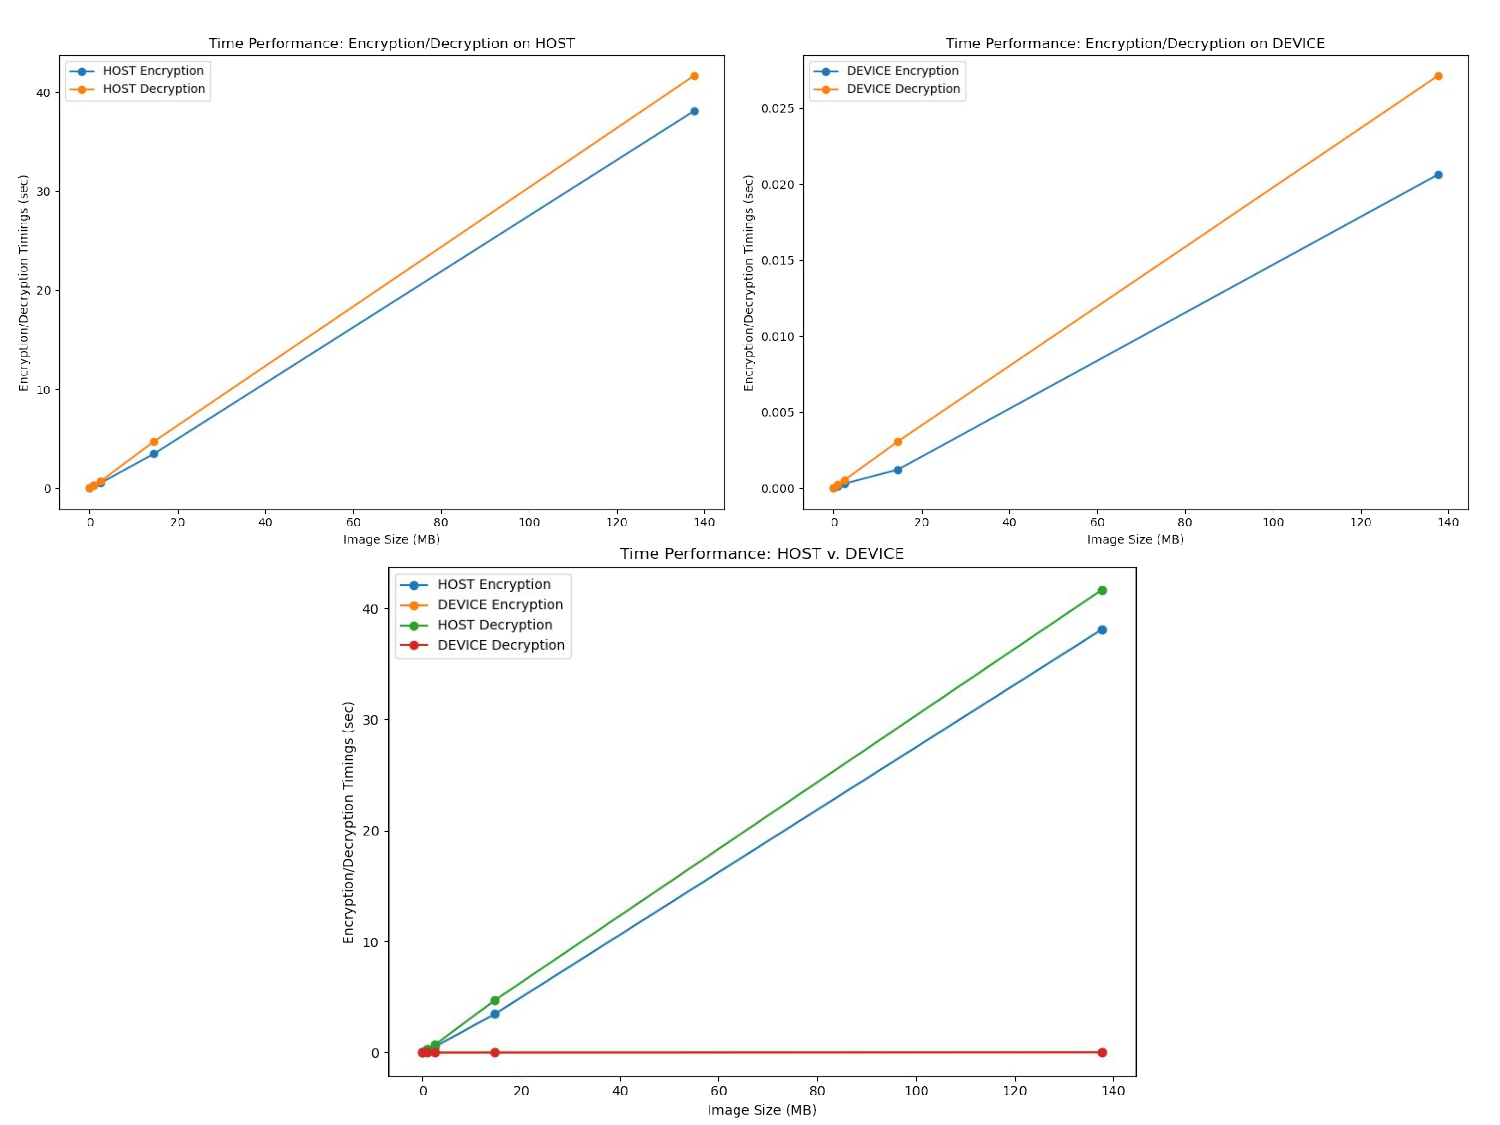
\includegraphics[scale=.8]{tex/Projects/CamdenLandis/timing_plots.pdf}}
\caption{Comparison plots of HOST and DEVICE timings.}
\label{fig}
\end{figure}

\begin{figure}[!ht]\centering
\makebox[\textwidth][c]{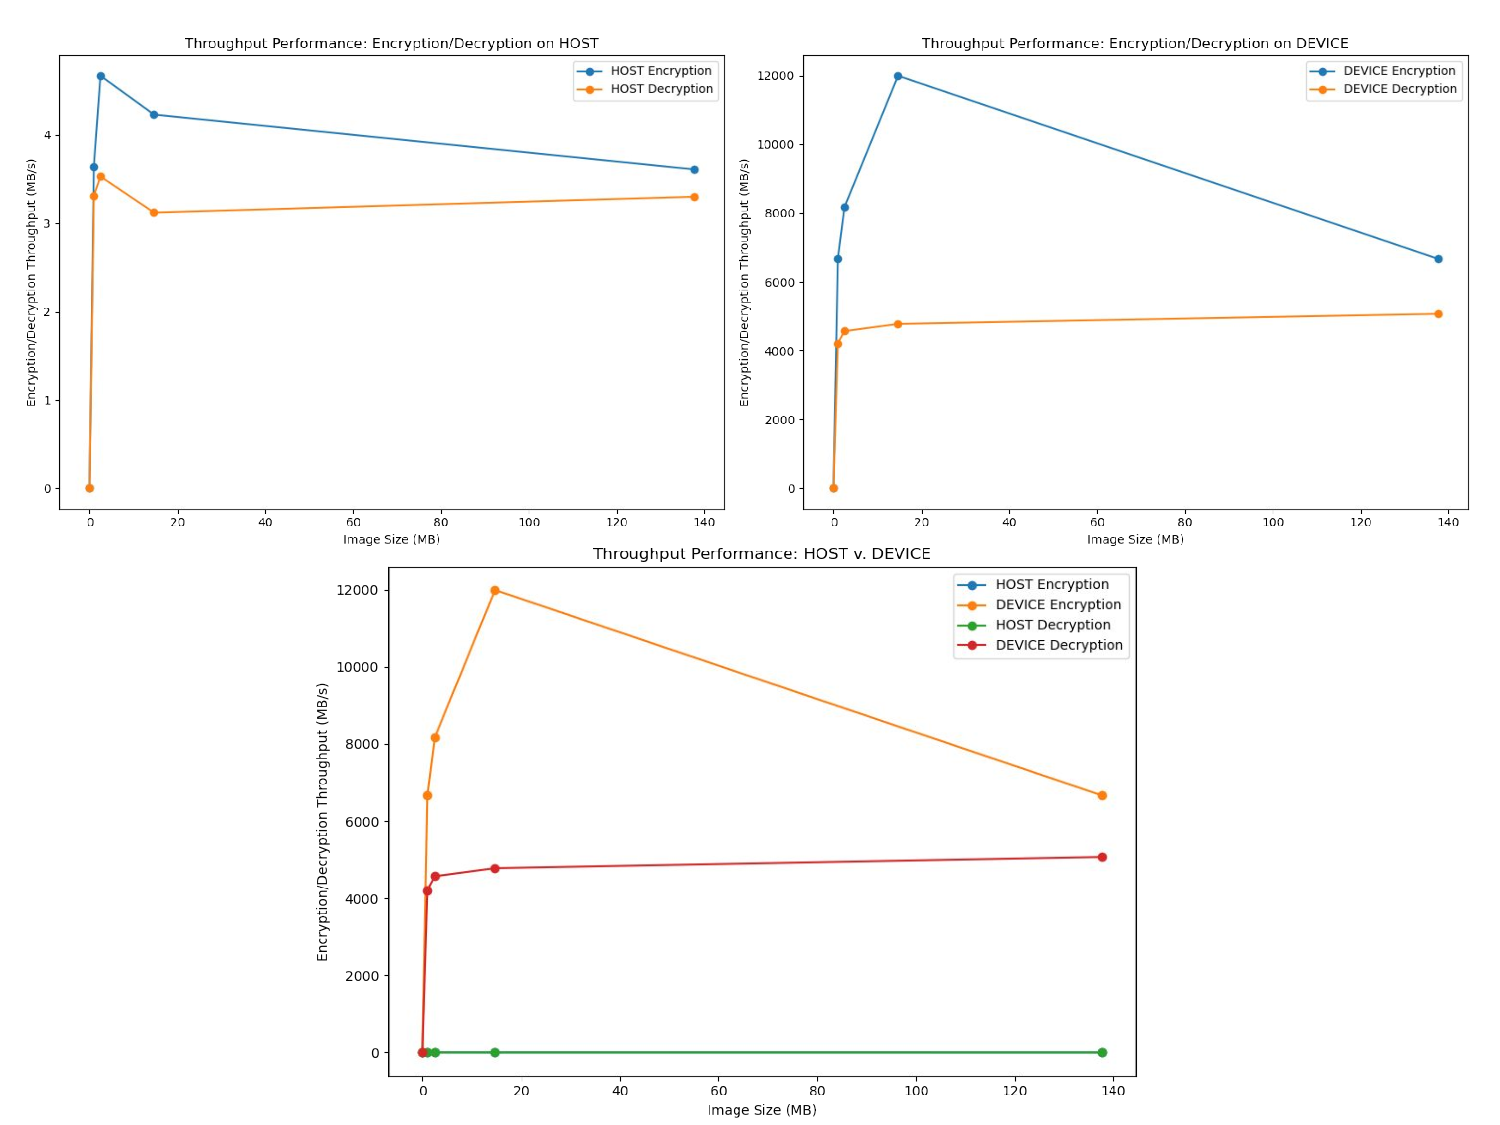
\includegraphics[scale=.8]{tex/Projects/CamdenLandis/throughput_plots.pdf}}
\caption{Comparison plots of HOST and DEVICE timings.}
\label{fig}
\end{figure}

Though it appears that in Figure 1.3 there is some plateauing and drop off when using the encryption kernel, the parallel implementation dominates the serial implementation (which may not be an entirely fair claim given that the serial code is not optimized).

\section{Visual Example}

Figure 1.4 shows the encryption and decryption outputs of a single bitmap image:

\vspace{-0.3in}
\begin{figure}[!ht]\centering
\makebox[\textwidth][c]{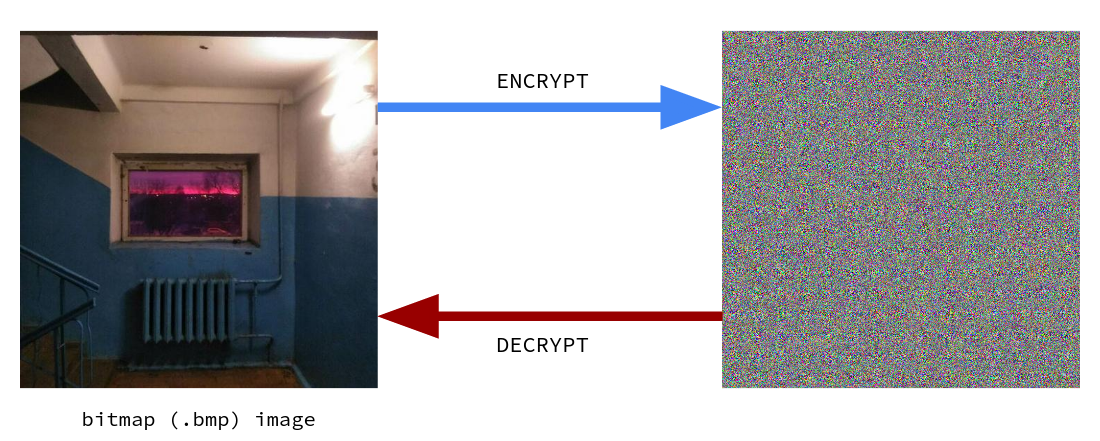
\includegraphics[scale=.35]{tex/Projects/CamdenLandis/example.png}}
\caption{Example bitmap image being processed with CUDA AES kernels.}
\label{fig}
\end{figure}

\newpage
\section{Future Implementation Improvements}
\begin{itemize}
    \item Utilizing the device's CUDA Tensor Cores for fused matrix multiply-add operations.
    \item Parallelizing the standard \texttt{bimap.c} source code for potentially faster data transfer with \texttt{cudaMemcpy}.
    \item Storing S-Box and round key arrays in shared memory.
    \item Implementing a batch image kernel for increasing the number of images being processed.
\end{itemize}

\section{Known Issues}
\begin{itemize}
    \item Depending on the device architecture, this software implementation may not operate correctly.
    \item The naive implementation of the parallel DEVICE encryption and decryption kernels do not encode or decode the entire image; shared memory kernels are used instead.
\end{itemize}

\section{Outcomes}
The main point of this project was to take a known cryptographic algorithm, research how others have parallelized code implementations of the algorithm, and then try to model my own version. Though my current implementation is far from being perfectly optimized, I did successfully show that my AES kernels can be used to accelerate the image encryption/decryption process using nothing more than NVIDIA silcon, CUDA, and some haphazard coding practices. 

Looking at the basic time and throughput comparisons, I obtained upward of approximately 2,000 times higher throughput on the GPU when compared to CPU-only execution. This certainly shows that GPUs can be used for efficient image processing and encryption.

\hrulefill
